\documentclass[12pt,a4paper]{article}
\usepackage[spanish,es-tabla]{babel}
\usepackage{bbm}
\usepackage[utf8]{inputenc}
\usepackage{multicol}
\usepackage[T1]{fontenc}
\usepackage{graphicx}
\usepackage{gensymb}
\usepackage{amssymb, amsmath} %Paquetes matemáticos de la American Mathematical Society
\parskip=1 mm
\oddsidemargin -0.8 cm
\headsep -2 cm
\textwidth=17.8cm
\textheight=25.5cm
\begin{document}
\title{Laboratorio de Mecánica, Practica 5 - Movimiento Rectilíneo Uniforme}
\date{12 de marzo del 2025}
\author{\textbf{Ortega Montero Fernando Naed} - Equipo 4\\
Yibran Morales Munguía\\
Victor Manuel Santillan Romero}
\maketitle
\section{Resumen} 

En este informe de laboratorio se exponen tres experimentos sobre movimiento rectilíneo uniforme analizados con tres distintos métodos, fotocompuetas, fotografía estroboscópica y grabación de video, estos últimos dos analizados con el software “Traker”; así mismo para estos últimos dos se realiza la obtención de un modelo ideal por regresión lineal usando los datos experimentales.

\section{Introducción}

El movimiento rectilíneo uniforme (MRU) es el movimiento de un objeto con velocidad constante a lo largo de una recta, esto implica la ausencia de toda fuerza externa. Donde la posición de un objeto con respecto al tiempo sigue la ecuación…
\[x(t) = t v + x_0\]
Donde…\\

\noindent$t$ : tiempo, en segundos (s).\\
 $v$ : velocidad, en metros sobre segundo ($\frac{m}{s}$).\\
$x_0$ : posición inicial, en metros (m).\\
$x(t)$ : posición del objeto en un tiempo $t$, en metros (m).\\

Como se puede notar esta ecuación tiene la forma de la ecuación de una recta, donde $v = m$, entonces podemos calcular $v$ con…
\[v = \frac{x_2 - x_1}{t_2 - t_1}\]
Con $(x_1, t_1), (x_2, t_2)$ como puntos de la recta.\\

Por otra parte se tendrá que hacer referencia a los siguientes conceptos en fotografía: \\

El diafragma: es la pieza de la cámara que regula la cantidad de luz que entra en el lente; se denotará como $D$.\\

El obturador: La pieza de la cámara que regula la cantidad de tiempo que el lente es expuesto a la luz, esta variable es importante ya que con un tiempo de exposición alto los objetos en movimiento se verán desplazados, dejando sus posiciones anteriores como parte de la imagen; se denotará como $t_c$.\\

La sensibilidad: mide la capacidad del sensor de la cámara para captar luz, cuanto menor sea la capacidad de captar luz las imágenes serán mas obscuras, cuanto mayor sea las imágenes serán mas claras; se denotará como ISO.\\

$f$: es la razón entre la distancia focal y la apertura del obturador ($\frac{F}{D} = f$, con F como la distancia focal y D como la apertura del obturador) de esto sigue que con un diámetro de apertura del obturador muy pequeño se tiene menor cantidad de luz pero un mejor enfoque y con un diámetro de apertura del obturador mas grande se tiene una mayor cantidad de luz pero un peor enfoque.

\section{Desarrollo experimental}

Para el primer ejercicio se empleo un riel de aire, una compresora de aire, un carro para riel, dos fotocompuertas conectadas a un Smart Timer (con precisión de 0.0001 s), un flexometro (con una precisión de 0.1 cm)  y un nivel.\\
Se colocó el riel de aire en el suelo, se niveló para que no hubiera ninguna fuerza fuera de las deseadas actuando sobre el carro, se colocaron las fotocompuetas a 150.0 cm una de la otra.\\
Después se midieron seis tiempos en los cuales el carrito recorrió los 150.0 cm, con velocidades diferentes.\\

Para el segundo ejercicio se utilizó un riel de aire, una compresora de aire, un carro para riel, un tripie, una cámara fotográfica, un nivel, un flexómetro (con una precisión de 0.1 cm) y una regla de madera de 2 m (con una precisión de 1 cm).\\
Se coloco el riel de aire nivelado sobre la mesa para descartar fuerzas no deseadas, se alineó la regla de madera a lo largo del riel, con esto se grabó el movimiento del carro a lo largo del riel; de un punto inicial a un punto final situados a 126.5 cm de distancia entre ellos, después de haber sido impulsado por una fuerza arbitraria.\\

El tercer ejercicio se utilizó un riel de aire, una compresora de aire, un carro para riel, una regla de 2 m (con una precisión de 1 cm), un nivel, plastilina, un alambre, dos tripies, un estroboscopio marca Fluke y una cámara fotográfica.\\
Se colocó el riel horizontal y nivelado, se colocó la cámara en un tripie y se ajusto a la altura del riel de aire, se colocó el estroboscopio en el otro tripie y se tomó una frecuencia fija, al carro se le adapto una pequeña antena con la plastilina y un alambre, para así poder saber su posición en cada destello de luz emitido por el estroboscopio.\\

Con esto montado, tomamos la cámara ajustamos el tiempo de exposición, los destellos por minuto, el ISO, y la distancia focal, usando el temporizador de la cámara, para no tener vibraciones indeseadas, se toma una foto del movimiento del carro a lo largo del riel, con las variables ajustadas adecuadamente la foto podrá captar la posición del carro a lo largo del riel en cada destello de luz emitido por el estroboscopio.\\

Finalmente esta foto será tratada por el programa Tracker con el objetivo de encontrar las distancias entre cada punto capturado por la cámara, y con ayuda de la frecuencia del estroboscopio podremos obtener una tabla de posición contra tiempo, finalmente encontrando una ecuación de la recta que describa un modelo ideal.

\section{Resultados}

Los tiempos de la Tabla 1 fueron tomados impulsando el carro con una fuerza arbitraria tomando solo el intervalo de ida entre las dos fotocompuertas, este interbalo era de 1.500 m .\\

Los tiempos de la Tabla 2 fueron tomados impulsando el carro con una fuerza arbitraria y dejándolo rebotar entre un par de ligas situadas a 1.800 cm una de otra, y midiendo solo el intervalo de tiempo en el cual el carro recorrió los 1.500 cm; entre cada fotocompuerta (solo de ida como se midió en el ejercicio 1).\\

Las distancias y tiempos de la Tabla 3 fueron obtenidos grabando el movimiento de el carro a lo largo del riel de aire, usando el software Traker se analizó el video y se obtuvieron los datos.\\

Las distancias de la Tabla 4 fueron obtenidas usando el software Traker, analizando una fotografía tomada considerando las siguientes variables de la cámara, ISO = 400, tiempo de exposición 4 s, f = 5.0 y del estroboscopio 550 destellos por minuto.

\begin{table}[h!]
\begin{center}
\begin{tabular}{|c|c|c|c|}
\hline
No. & Tiempo (s) & Distancia (m) & Velocidad $(\frac{m}{s})$\\
\hline
1 & 2.6293 (0.0001) s & 1.500 (0.001) m & 0.5704 $\frac{m}{s}$\\
\hline
2 &  2.8373 (0.0001) s & 1.500 (0.001) m & 0.5286 $\frac{m}{s}$\\
\hline
3 & 2.7554 (0.0001) s & 1.500 (0.001) m &0.5443 $\frac{m}{s}$\\
\hline
4 & 3.0242 (0.0001) s & 1.500 (0.001) m &0.4959 $\frac{m}{s}$\\
\hline
5 & 1.5422 (0.0001) s & 1.500 (0.001) m &0.9726 $\frac{m}{s}$\\
\hline
6 & 1.7058 (0.0001) s & 1.500 (0.001) m &0.8793 $\frac{m}{s}$ \\
\hline
\end{tabular}
\caption{Tiempos producidos por una fuerza albitraria}
\end{center}
\end{table}

\begin{table}[h!]
\begin{center}
\begin{tabular}{|c|c|c|c|}
\hline
No. & Tiempo (s) & Distancia (m) & Velocidad ($\frac{m}{s}$)\\
\hline
1 & 1.1176 (0.0001) s & 1.500 (0.001) m & 1.3421 $\frac{m}{s}$ \\ \hline 
2 & 1.4441 (0.0001) s & 1.500 (0.001) m & 1.0387 $\frac{m}{s}$ \\ \hline  
3 & 1.7720 (0.0001) s & 1.500 (0.001) m & 0.8465 $\frac{m}{s}$ \\ \hline  
4 & 2.1518 (0.0001) s & 1.500 (0.001) m & 0.6970 $\frac{m}{s}$ \\ \hline 
5 & 2.5948 (0.0001) s & 1.500 (0.001) m & 0.5780 $\frac{m}{s}$ \\ \hline
6 & 3.1171 (0.0001) s & 1.500 (0.001) m & 0.4812 $\frac{m}{s}$ \\ \hline  
7 & 3.7396 (0.0001) s & 1.500 (0.001) m & 0.4011 $\frac{m}{s}$ \\ \hline 
8 & 4.4658 (0.0001) s & 1.500 (0.001) m & 0.3358 $\frac{m}{s}$ \\ \hline
9 & 5.3694 (0.0001) s & 1.500 (0.001) m & 0.2793 $\frac{m}{s}$ \\ \hline 
10 & 6.4624 (0.0001) s & 1.500 (0.001) m & 0.2321 $\frac{m}{s}$ \\ \hline 
11 & 7.7637 (0.0001) s & 1.500 (0.001) m & 0.1932 $\frac{m}{s}$ \\ \hline 
\end{tabular}
\caption{Tiempos producidos por la ocilación del carro entre las ligas}
\end{center}
\end{table}

\begin{table}[h!]
\begin{center}
\begin{tabular}{|c|c|c|}
\hline
No. & Tiempo (s) & Distancia (m) \\ \hline 

1 & 0.034 s & 0.0072 (0.0010) m \\ \hline 
2 & 0.068 s & 0.0118 (0.0010) m \\ \hline 
3 & 1.002 s & 0.0164 (0.0010) m \\ \hline 
4 & 1.336 s & 0.2098 (0.0010) m \\ \hline 
5 & 1.670 s & 0.2572 (0.0010) m \\ \hline 
6 & 2.004 s & 0.3042 (0.0010) m \\ \hline 
7 & 2.338 s & 0.3524 (0.0010) m \\ \hline 
8 & 2.672 s & 0.4003 (0.0010) m \\ \hline 
9 & 3.006 s & 0.4508 (0.0010) m \\ \hline 
10 & 3.340 s & 0.5022 (0.0010) m \\ \hline 
11 & 3.674 s & 0.5513 (0.0010) m \\ \hline 
12 & 4.008 s & 0.6005 (0.0010) m \\ \hline 
13 & 4.342 s & 0.6466 (0.0010) m \\ \hline 
14 & 4.676 s & 0.6957 (0.0010)  m \\ \hline 
15 & 5.010 s & 0.7445 (0.0010) m \\ \hline 
16 & 5.344 s & 0.7910 (0.0010) m \\ \hline 
17 & 5.678 s & 0.8384 (0.0010) m \\ \hline 
18 & 6.012 s & 0.8818 (0.0010) m \\ \hline 
19 & 6.346 s & 0.9256 (0.0010) m \\ \hline 
20 & 6.680 s & 0.9757 (0.0010) m \\ \hline 
21 & 7.014 s & 1.0195 (0.0010) m \\ \hline 
22 & 7.348 s & 1.0630 (0.0010) m \\ \hline 
23 & 7.682 s & 1.1095 (0.0010) m \\ \hline 

\end{tabular}
\caption{Distancias obtenidas bajo intervalos de tiempos fijos.}
\end{center}
\end{table}

\begin{figure}[h!]
\centering
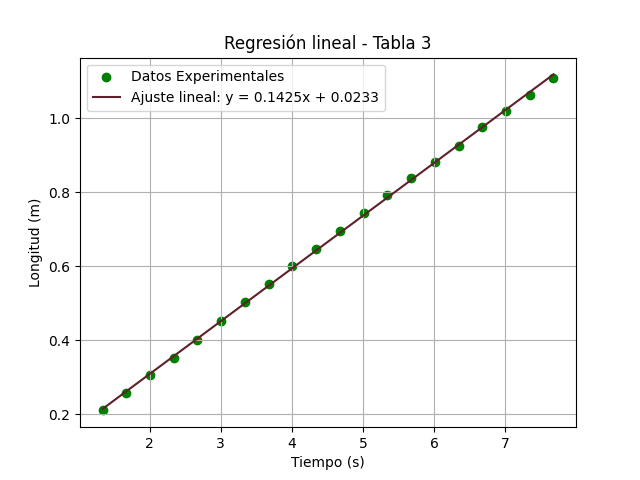
\includegraphics[scale=0.9]{Figure_3.png}
\end{figure}

\begin{table}[h!]
\begin{center}
\begin{tabular}{|c|c|c|}
\hline
No. & Tiempo (s) & Distancia (m) \\
\hline
1  & 0.00012 s & 0.0867 (0.013) m \\ \hline 
2  & 0.00024 s & 0.1744 (0.013) m \\ \hline 
3  & 0.00036 s & 0.2628 (0.013) m \\ \hline 
4  & 0.00048 s & 0.3490 (0.013) m \\ \hline 
5  & 0.00060 s & 0.4367 (0.013) m \\ \hline 
6  & 0.00072 s & 0.5229 (0.013) m\\ \hline 
7  & 0.00084 s & 0.6121 (0.013) m\\ \hline 
8  & 0.00096 s & 0.6998 (0.013) m \\ \hline 
9 & 0.00108 s  & 0.7867 (0.013) m \\ \hline 
10  & 0.00120 s & 0.8729 (0.013) m \\ \hline 
\end{tabular}
\caption{Distancias obtenidas bajo intervalos de tiempos fijos.}
\end{center}
\end{table}

\begin{figure}[h!]
\centering
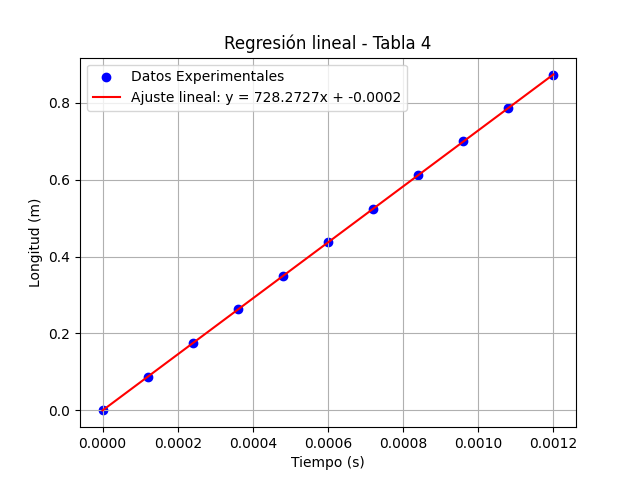
\includegraphics[scale=0.9]{Figure_4.png}
\end{figure}

\newpage
.

\section{Discusión}

Debido a que en la Tabla 1 y 2 solo la variable del tiempo cambia no es posible hacer una gráfica, y solamente se calcula el valor de la velocidad siguiendo la siguiente formula:
 \[ V = \frac{d}{t}\]
Como se puede notar en la Tabla 3, solo las distancias tienen incertidumbre esto se debe a que son datos obtenidos del análisis con el software Traker, este no marca una incertidumbre para el tiempo, pero si podemos dar una para la distancia debido a que la colocación de las masas puntuales dentro del software es manual, por lo que se puede obtener una incertidumbre de 0.0010 m, esto se obtiene de la diferencia de la distancia entre el inicio y el final de un pixel que es parte del final del carro en el video.\\
En la Tabla 4 se puede notar que solo hay incertidumbre en la distancia, esto ocurre por una razón similar a la de la Tabla 3, el Traker toma una diferencia de posición entre el inicio y el final de la marca; que denota la posición del carro en cada destello de la luz, de 0.013 m por lo que esa será la incertidumbre de la distancia.\\

Como se puede notar en las gráficas de las Tablas 3 y 4, los datos experimentales realmente son muy cercanos a el modelo ideal de un movimiento rectilíneo uniforme, aun si estos varían con la incertidumbre. 

\section{Conclusión}

Como se mencionó en la discusión el gran parecido de los datos experimentales con la recta ideal puede indicar que los ejercicios 2 y 3 fueron correctamente realizados, reduciendo al mínimo los efectos de fuerzas externas no deseadas que podrían producir una aceleración y por lo tanto un movimiento rectilíneo acelerado. 
 Finalmente el uso de herramientas como Traker facilita enormemente el análisis del movimiento de objetos tanto de videos como de fotografías estroboscópicas, el único problema es que no especifica la incertidumbre del tiempo. 


\section{Referencias}

Martín, J. M. (2025) \textit{Física Experimental. Introducción a los conceptos y métodos.} Recuperado el 11, 02, 2025, de https://copitarxives.fisica.unam.mx/LT0006ES/LT0006ES.pdf \\

García J. (1977)  \textit{Mira y fotografía :   aprende a usar tu cámara para crear las fotografías que imaginas} Barcelona :   Editorial GG\\




\end{document}